\begin{figure}
	\centering
	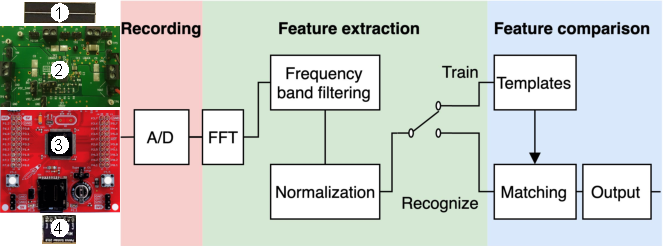
\includegraphics[width=\columnwidth]{figures/cis}
	\caption{Coalesced Intermittent Command Recognizer: an instant of a \fullsys. On the left is the hardware of an individual intermittent sensory node. Our prototype consists of 8 coalesced intermittent nodes. \circled{1} is an SLMD121H04L solar panel. \circled{2} is a BQ25570EVM-206 solar power harvester, \circled{3} is an MSP430FR5994 ultra low power microcontroller, and \circled{4} is a home soldered PCB with KPMM-3738-VM1010-R microphone. The block diagram on the right shows the data acquisition and processing stages.}
	\label{fig:cis}
\end{figure}

We have developed a prototype of a \fullcim (\cim): an instant of a \fullsys. The reason behind developing a \cim is threefold: (i) voice is a natural and convenient way for human to interact with miniaturized devices; (ii) By demonstrating \textit{the world's first} \fullcim, we are shading light on the potential of intermittent systems; and (iii) it facilitates testing with different sensing strategies and with different type of external events arrival (i.e. regular  or burst). 

We envision that a \cim can be embedded in clothes, walls, wallpapers, and furniture coverage. \cim can enable local communication by taking advantage of the recent advancements in passive communication (\cite{marco} shows 60\,m distance of direct passive light communication). 

\subsection{Hardware}
A \cim node consists of thee main parts: a microphone, a microcontroller, and a harvester. we used MSP430RF5994~\cite{ti_msp430_website} an ultra-low-power microcontroller for data acquisition and processing. This microcontroller has a 16-bit RISC processor running on 1 MHz, 8KB of SRAM (volatile), 256KB of FRAM (non-volatile), and a 12-bit analog to digital converter (ADC). It also features a Low Energy Accelerator (LEA), which offloads the main CPU for specific operations, such as FFT. For recording we used the PMM-3738-VM1010-R piezoelectric MEMS microphone, which features Wake on Sound and ZeroPower listening technologies \cite{microphone}, allowing both the microcontroller and the microphone to sleep in a low-power mode until a sound is detected.
The microcontroller and microphone are powered by a BQ25570 solar power harvester~\cite{BQ25570EVM-206_website} connected to an IXYS SLMD121H04L solar cell~\cite{SLMD121H04L_website} and a super-capacitor of 220 \si{\micro F}. For debugging we used the Saleae logic analyzer~\cite{saleae}.

\subsection{Data acquisition}
To cover the frequency range of the human voice, we used a sample rate of 7,812 Hz. To determine the location of the word within the recorded signal, we relied on the microphone feature  \textit{Wake-on-sound} and on the characteristics of the targeted vocabulary. The wake-on-sound triggers the data recording on the beginning of a word---once the energy in the sound wave crosses a certain level the recording begins. Experimentally, we defined the effective recoding length to be 259\,ms. Thus, endpoint detection algorithm is not needed, greatly improving the processing time and system efficiency from the energy perspective. Once a recording has finished, framing and data processing begin. We used non-overlapping frames of 256 samples ($\approx$ 33 milliseconds). This size is beneficial for doing a Fast Fourier Transform and short enough for the voice-features to be considered constant inside one frame.

% \begin{figure}
% 	\centering
% 	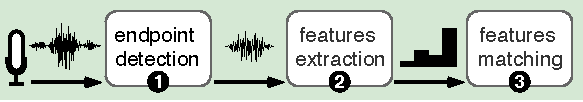
\includegraphics[width=\columnwidth]{figures/distributedMicrophone}
% 	\caption{ (1) endpoint detection algorithms extract the part of the signal corresponds to the input word, (2) feature extraction calculates the energy spectrum of the trimmed signal, and (3) feature matching searches the local database for the closest word}
% 	\label{fig:mic}
% \end{figure}

\subsection{Software}
We have developed a power interrupt immune word recognizer. Figure~\ref{fig:cis} shows its main modules with are explained below. 

\subsubsection{Feature Extraction}
Once the position of a word is determined, features of the recorded voice are extracted for comparison against previously stored templates. Feature extraction takes place on a frame-by-frame basis and is based on the energy and spectral characteristics of each frame. The spectral characteristics of a frame are determined by dividing the frequency range of interest into several spectral bands. We used 12 spectral bands as in~\cite{Hopper1992}. %(\ref{tab:bands}).
Because most of the energy in human speech is contained in lower frequencies, the width of the bands is smaller for the lower frequencies and gradually gets bigger as the frequency gets higher.

%Using spectral bands that are sized this way also makes them have a more equal range size according to the Mel scale~\cite{Stevens1937}.

%\subsubsection{Fast Fourier Transform}
For each frame in a word, a 256-point FFT is performed. The results of the FFT are used to determine the energy in each of the 12 spectral bands. This process essentially produces a 12-element vector for each frame of the speech input. Each element of the vector represents the energy in one of the 12 spectral bands. These vectors will become the basis for comparison against the previously stored templates, once they are normalized.


% \begin{table}[]
% \centering
% \caption{Spectral bands used for feature extraction. }
% \label{tab:bands}
% \begin{tabular}{c c}
% \hline
% Band & Frequency range (Hz) \\ \hline
% 1    & 100-300    \\
% 2    & 250-450    \\
% 3    & 400-600    \\
% 4    & 550-750    \\
% 5    & 700-900    \\
%  & \\
% 6    & 900-1200   \\
% 7    & 1200-1500  \\
% 8    & 1500-1800  \\
%  & \\
% 9    & 1800-2300  \\
% 10   & 2300-2800  \\
%  & \\
% 11   & 2800-3400  \\
% 12   & 3400-4000  \\ \hline
% \end{tabular}
% \end{table}

\paragraph{Normalization}
Once the features are extracted from the speech input, the frames are normalized. This process helps to eliminate detection errors that could result from differences in the amplitude of the speech input of a word. To normalize a feature vector, for each of the spectral bands the binary logarithm is taken of the energy in that band and the average energy logarithm of the frame is subtracted from that. This is shown in the following equation:
\begin{equation}
    f_i = \log(\hat{f}_i) - \frac{\sum\limits^S_{i=1}\log(\hat{f}_i)}{S},
\end{equation}
where $f_i$ is the normalized output for the $i^{\text{\tiny th}}$ spectral band of the frame. $\hat{f}_i$ is the energy in the $i$th spectral band of the frame and $S$ is the number of spectral bands (12 in our case).

\subsubsection{Feature Matching}
The system identifies the recorded word by comparing the normalized features of the input signal against the features of all the templates contained in its dictionary.

The similarity between two frames is determined by computing the distance between them, which can be obtained by computing the squared Euclidean distance between their normalized vectors as shown in the following equation:
\begin{equation}
    {\rm d}[F_T, F_R] = \sum\limits^S_{i=1} (f_{T,i} - f_{R,i})^2,
    \label{eq:frame_dist}
\end{equation}
where d is the the distance between two frames, $F_T$ is the a template frame, $F_R$ is the a recorded frame, $f_{T,i}$ is the normalized output of the $i^{\text{\tiny th}}$ spectral band of a template frame, $f_{R,i}$ is the normalized output of the $i^{\text{\tiny th}}$ spectral band of a recorded frame and $S$ is the number of spectral bands.


\paragraph{Linear Distance Matching}
\label{sec:LDM}
In Linear Distance Matching (LDM) the frames within the feature vectors of two words are compared successively, not accounting for differences in pronunciation speed. LDM can only compare feature vectors of equal length.
The total distance between two words is calculated as follows:
\begin{equation}
{\rm d}[W_T, W_R] = \sum\limits^{L}_{i=1} {\rm d}[F_{T,i}, F_{R,i}],
\end{equation}
where d is the distance, $W_T$ is a template word, $W_R$ is a recorded word,  $F_{T,i}$ is the $i^{\text{\tiny th}}$ template frame, $F_{R,i}$ is the $i^{\text{\tiny th}}$ recorded frame, and $L$ is the recording length measured in frames.


% During \textit{feature extraction} on frames containing the word Fast Fourier Transform is applied to obtain the energy spectrum. 
% The energy spectrum is then sorted into a feature vector, where each vector value holds the total energy of a specific frequency range. Finally each vector value is normalized over the total vector energy.

% After that, \textit{feature matching} is performed, where the features of the recorded word are compared against a local database to find the most similar word in the database.
% There exist many feature matching methods, yet only few are able to run under the constraints of an intermittent system.
% Two methods have been implemented and tested. The first is Dynamic Time Warping (DTW), which is able to compare two sequences of data, even when they vary in speed. This way if a word is spoken slower or faster, the algorithm can compensate for that.
% The second is a method that linearly compares two feature vectors. This requires less computations than DTW.


% \subsection{Implementation}
% During recording a sample rate was used of 7812 Hz, which covers the human voice frequency range. The used frame size was 256 samples. This size was beneficial for doing a Fast Fourier Transform and corresponds to approximately 33 milliseconds of speech.

% For normalization an integer log function was applied on every value, divided by the average log.
% The whole algorithm is implemented using only integer / fixed point arithmetic.

% %DTW is a well known method in speech recognition.
% In the linear comparing method the feature vectors of two words are compared successively, not accounting for differences in the speed of pronunciation. If two words vary in length, the last frames cannot always be compared and instead a penalty is applied linear to the length difference.

% In between the different steps (see figure \ref{fig:mic}) checkpoints in non-volatile memory are used to assure progress while running on intermittent power. In some cases additional checkpoint were used inside the steps.

